\printMiniToc



\textit{Dans cette partie, j'expliquerai les détails de l'univers du jeu mais aussi les raisons qui m'ont poussé à faire les choix qui y ont mené. Il est à noter que l'univers n'est pas terminé; s'il suffit largement aux besoins du jeu, il pourrait, dans l'optique de la réalisation d'une version complète, être agrandi et complété. De plus, certains détails, exprimés dans ce texte, dépassent déjà largement la portée de la démo.}



\section{Les thèmes importants}
Comme je l'ai déjà indiqué dans la section \ref{sec:objectifsTM}, ce jeu est l'occasion pour moi de développer des thématiques qui me porte à c\oe ur. C'est un jeu d'opinion qui se veut le défenseur de certains points de vue, les miens. Le jeu évolue donc autour de quelques thématiques clés, chères à mes yeux.

Le point le plus important est la relation humaine à la Nature. J'ai toujours été fasciné par sa beauté, sa cruauté, à la fois son ordre parfait et son désordre total. Pour moi, un retour à la Nature est une condition nécessaire pour atteindre le bonheur. La relation que nous entretenons avec elle, collaborative ou dominante, sera donc au c\oe ur du jeu et ce choix déterminera de nombreux aspects de l'histoire et du gameplay\definition.

Il existe cependant de multiples contradictions entre ma passion pour la Nature et l'univers qui m'entoure. Comment ne pas constater les dégâts que nous infligeons à notre environnement? Mais plus encore, comment ne pas constater que notre mode de vie (que certains nomment consumérisme) a perdu toute sa simplicité, son sens, sa \enquote{naturalité}! Ce jeu sera donc l'occasion de mettre le doigt sur ces paradoxes et l'opportunité de se poser certaines questions sur nos façons de faire.

Un autre thème conducteur sera la relation fraternelle (sororale dans le cas du jeu); sujet important à mes yeux, étant donné que j'ai moi-même un frère. Le jeu gravitera autour de la question de l'utilisation bénéfique et responsable ou destructrice et irresponsable de la technologie, des améliorations qu'elle peut apporter ou des dommages qu'elle peut causer et des abus auxquels elle peut conduire. Finalement, la question de la religion sera abordée, bien que dans une moindre mesure: quelle utilité a-t-elle? à quelles dérives peut-elle mener?



\section{Un monde divisé entre deux peuples}
L'univers dans lequel se déroule le jeu, nommé \nomUnivers, est divisé entre deux peuples: les Humains et les \nomNaturels s.



\section{Les Humains}
Les Humains sont une faction terne, grise et soumise à un tyran: Lord Gaamon. Le despote, atteint de folie, a une peur viscérale de la Nature et a convaincu le reste de la population de sa nocivité. Ce peuple perdu et sombrant dans la peur a, pour sa plus grande majorité, oublié son histoire et exécute avec soumission les ordres de son maître. L'utilisation de technologies mécaniques, polluantes et brutales est monnaie courante et permet à cette faction de dominer les autres; mais cela ne peut se faire sans ravager l'environnement.

Ce peuple vit enfermé dans \nomVille, une ville énorme, entourée de hautes murailles. Personne ne sort de ses frontières, de peur d'être contaminé par la Nature. Les Humains représentent un peuple perverti, brutal, apeuré et aveugle.


\subsection{L'histoire d'un peuple}
\begin{wrapfigure}[12]{r}{.3\textwidth}
	\vspace*{-.8cm}
	\center
	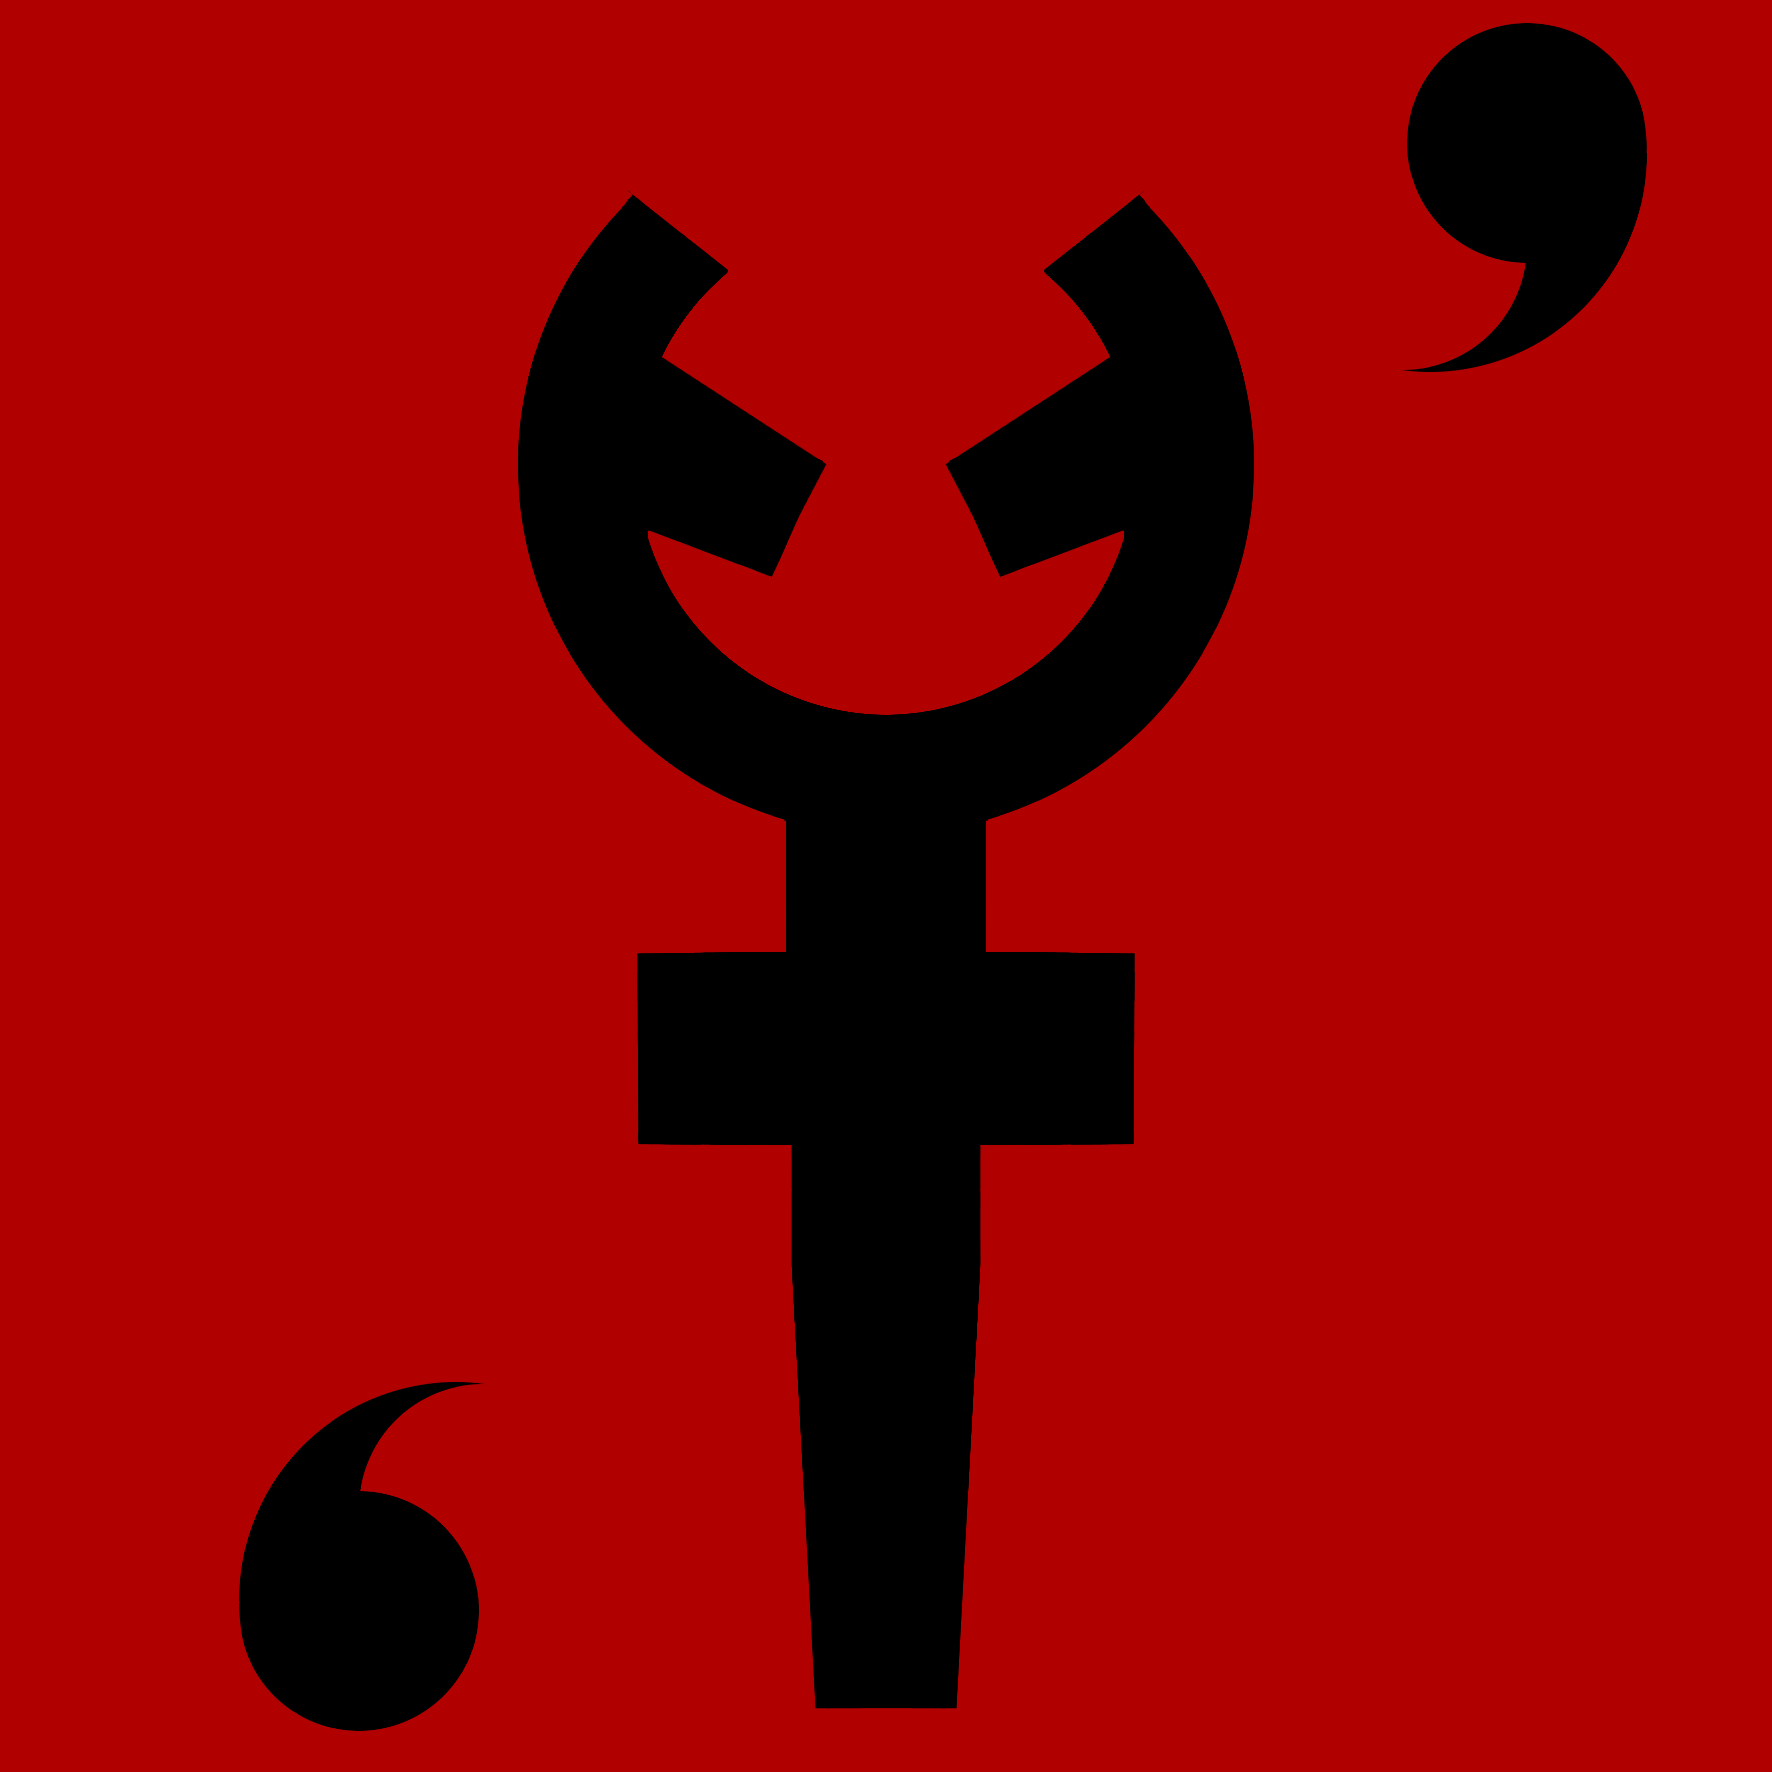
\includegraphics[width=\linewidth]{images/Monde/drapeauGaamon.png}
	\caption{Symbole de Gaamon}
\end{wrapfigure}

Quelques décennies avant le début du jeu, la ville était encore un petit village agréable. La vie agricole, bien que rude et laborieuse, y était appréciée et rares étaient les histoires qui venaient troubler la quiétude générale. Mais tout cela changea le jour où le jeune Gaamon arriva...

L'étranger, apparemment venu de contrées lointaines, décida de s'installer dans le bourg et fonda la première usine d'\nomUnivers. Son succès fut rapide: il apportait du travail et surtout produisait beaucoup grâce aux machines qu'il construisait. Il agrandit bientôt son usine... puis en construisit une deuxième. Grâce à cela, les conditions de vie s'améliorèrent, tout le monde avait du travail et la population était heureuse de cette venue providentielle.

Cela aurait pu rester ainsi pour de longues années, mais l'ambition de Gaamon était grande. Il fit construire d'autres usines, créa d'autres machines, employa bientôt tout le village et draina les populations des alentours dans ses halles de production. Les affaires allaient bon train, l'argent arrivait en quantité et son influence ne cessait de s'étendre.

Avec les années, il fédéra tous les Humains sous la bannière unique de ses usines et devint le maître incontesté de ce qui était devenu une ville. Mais Gaamon n'était pas complètement sain d'esprit; cachée au fond de lui résidait une folie, une phobie haineuse de la Nature. Le pouvoir et l'argent permirent à cette dernière, jusqu'alors refoulée, de s'exprimer de plus en plus pleinement et ouvertement. Il avait réussi à industrialiser, mécaniser le village, il voulait maintenant étendre son emprise hors des limites de la cité.

Il fortifia la ville en construisant des murailles et bâtit, en son centre, une immense tour d'acier et de verre qui devint l'icône emblématique de son empire. Il imposa à tous l'interdiction de sortir de l'enceinte des murs et brûla les dernières traces de verdure dans la cité. Il s'engagea alors, depuis le haut de sa nouvelle forteresse, dans un projet d'éradication plus vaste, qui annihilerait toute Nature, plantes ou animaux, des terres environnant les fortifications.

Le jeu débute quelques années après le commencement de ce funeste projet, à l'intérieur de la ville.


\subsection{La ville}

La ville est le bastion de la race humaine, l'empire de Lord Gaamon. Son décor relève de l'univers steampunk (voir annexe \ref{app:steampunk}). Il s'agit d'un monde urbain de l'ère industrielle où l'horizon est rythmé par les cheminées des hauts fourneaux qui crachent leur fumée nauséabonde et où la suie recouvre les architectures de métal et de verre. Cet environnement, métaphoriquement, représente l'utilisation abusive de la technologie. C'est aussi la haine envers la Nature, sa négation totale. Un plan de Murtos est donné à la figure \ref{fig:murtosLaGrande}.

\begin{figure}[h!]
	\hspace*{-2cm}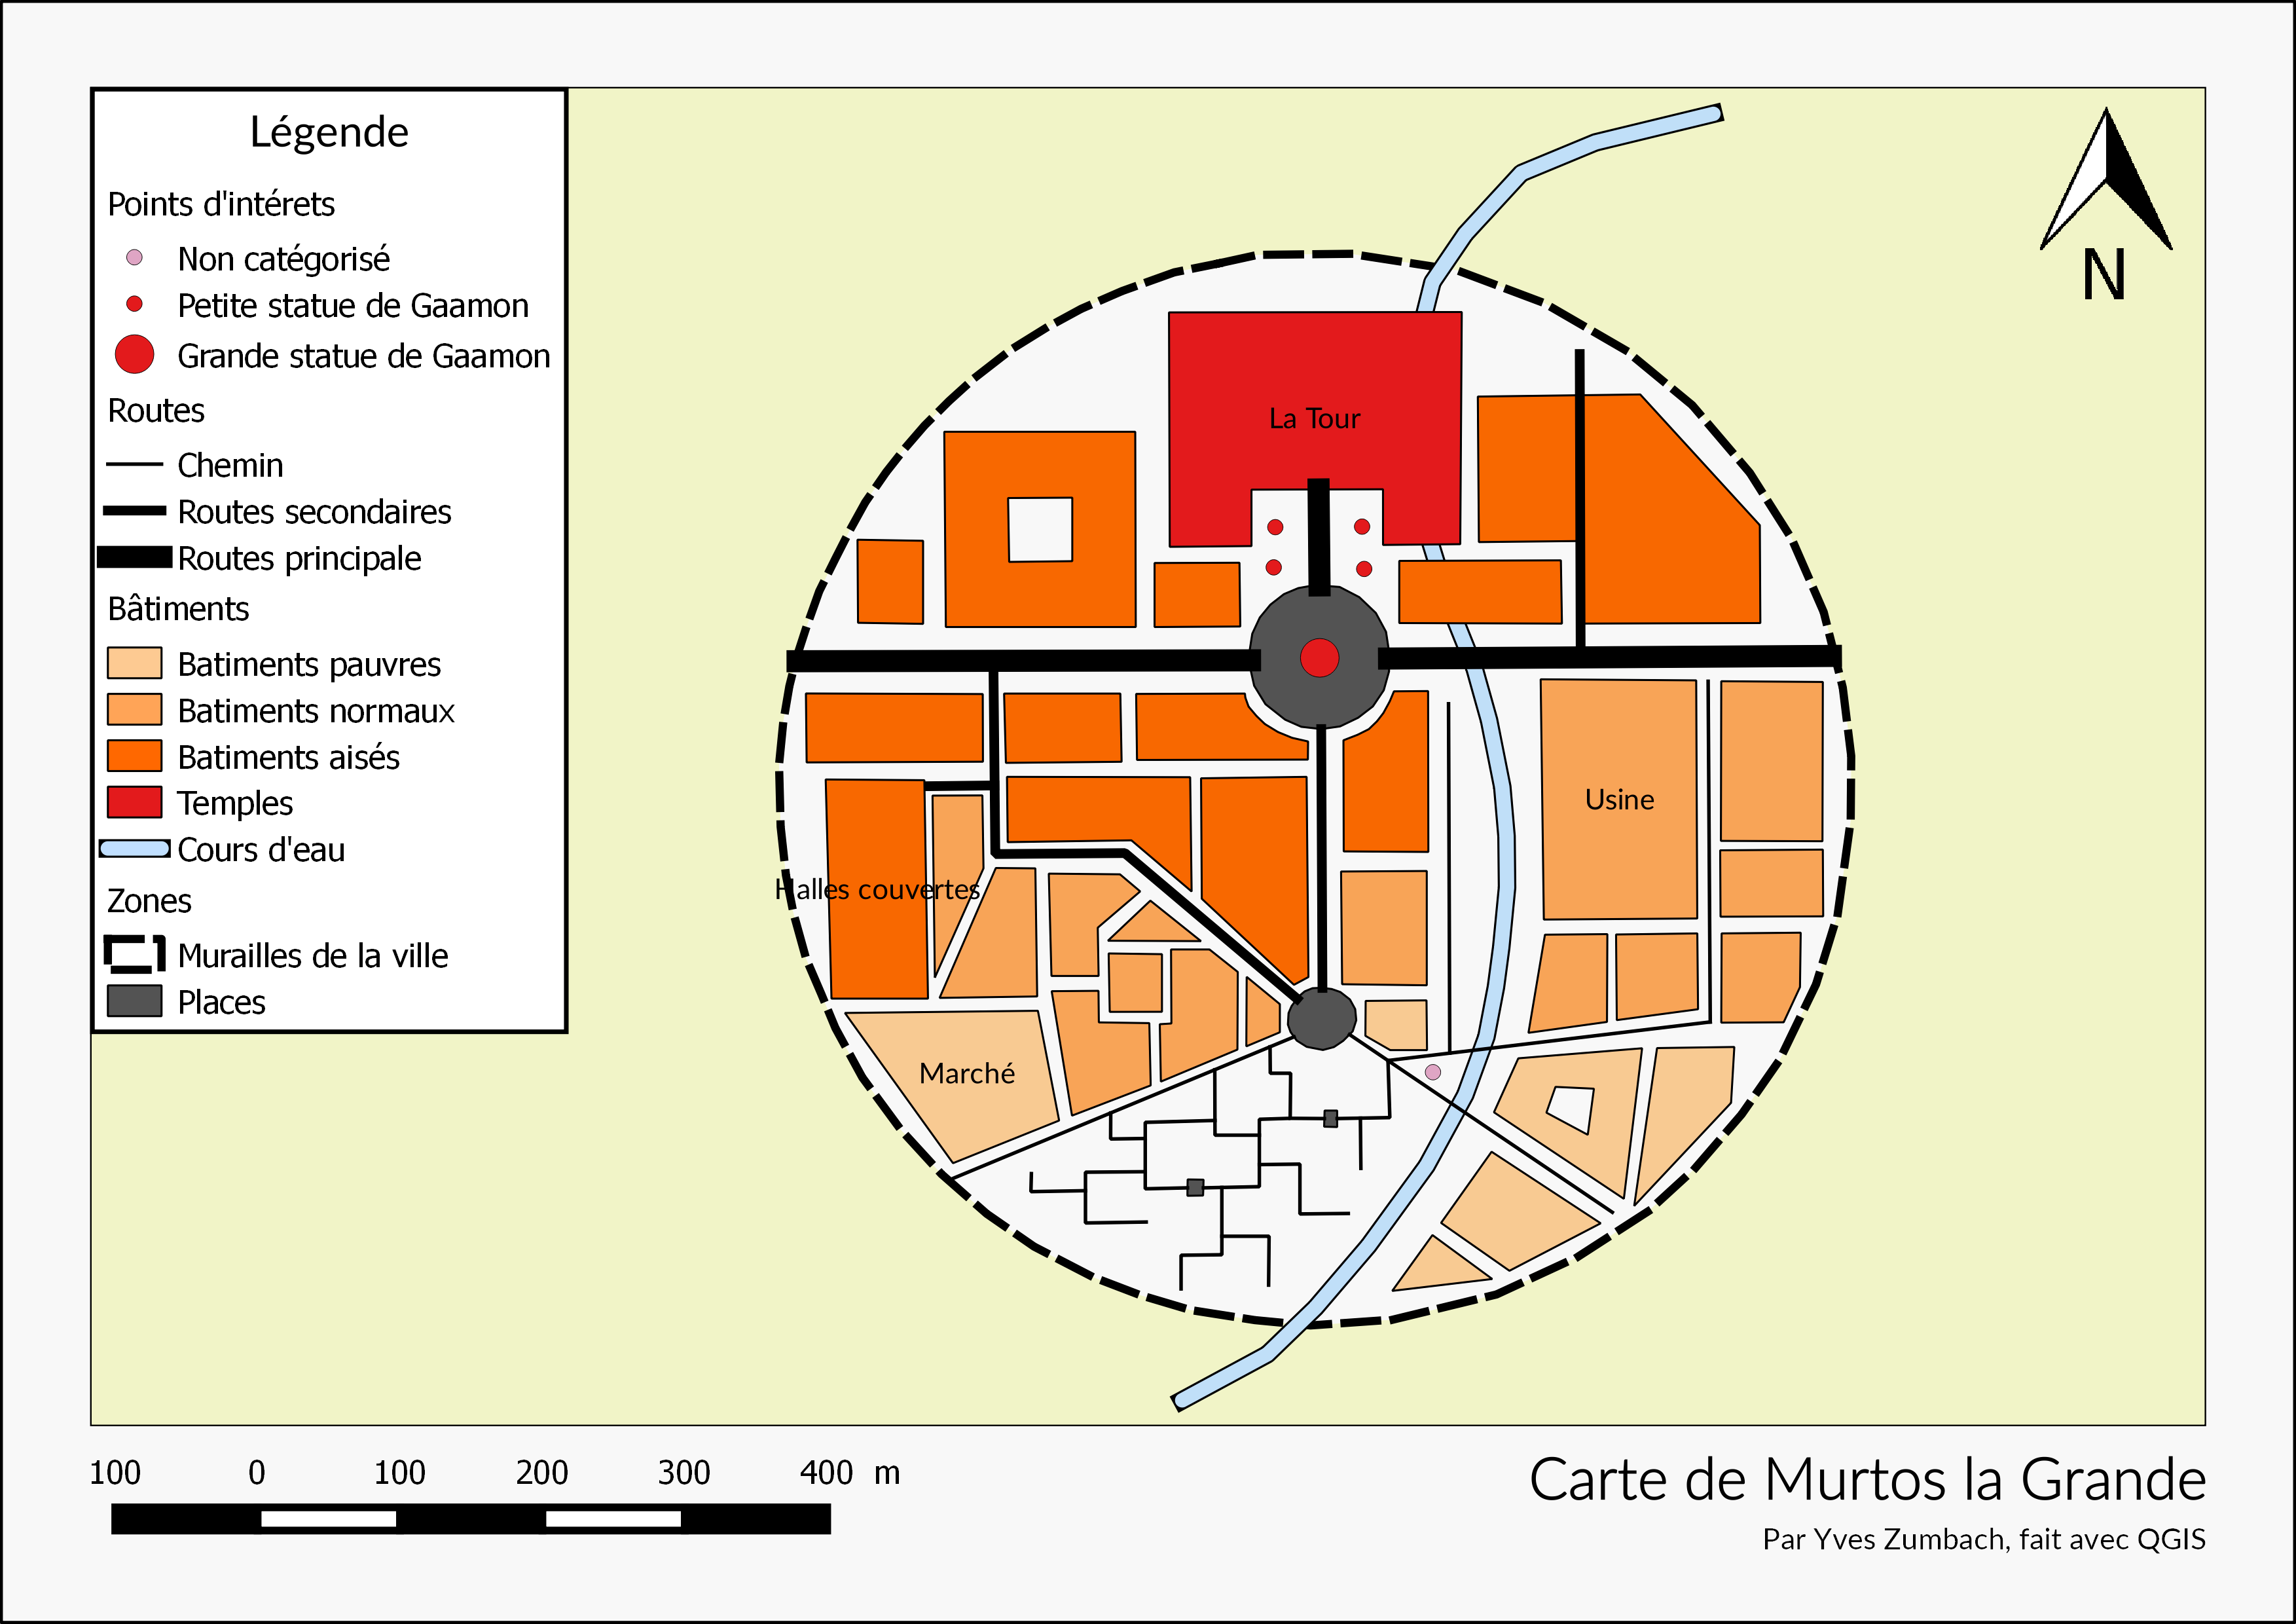
\includegraphics[width=\textwidth+2cm]{images/Monde/carteVille.png}
	\caption{Plan de la ville actuelle (Réalisé à l'aide du programme Quantum GIS)}
	\label{fig:murtosLaGrande}
\end{figure}



\subsection{La religion humaine}
La religion humaine est, à l'image de la ville, corrompue. Elle prône le bonheur par l'aisance matérielle, la richesse et la consommation. C'est même une apologie de la consommation -- si possible inutile -- que soutient ce dogme. De plus, comme les prêtres professent que l'argent ne s'acquiert que par le travail, Gaamon utilise la religion pour asservir les masses et motiver un travail acharné dans ses usines. Le symbole de ce culte possède une forme très caractéristique (voir figure \ref{subfig:accedeBonheur}) qui s'emboite avec l'icône de Gaamon pour représenter la collusion Religion--État. Quelques images de propagande que l'on peut trouver placardées sur les murs de la ville sont données par la figure \ref{fig:propagandeReligion}.

\begin{figure}[bh!]
	\subfloat[\label{subfig:accedeBonheur}Accède au Bonheur!]{
\includegraphics[width=.48\linewidth]{images/Monde/accedeAuBonheur.png}}
	\hspace*{.04\linewidth}\subfloat[Consommer pour la santé]{
\includegraphics[width=.48\linewidth]{images/Monde/consommerPourSante.png}}
	
	\subfloat[La Richesse c'est le Bonheur!]{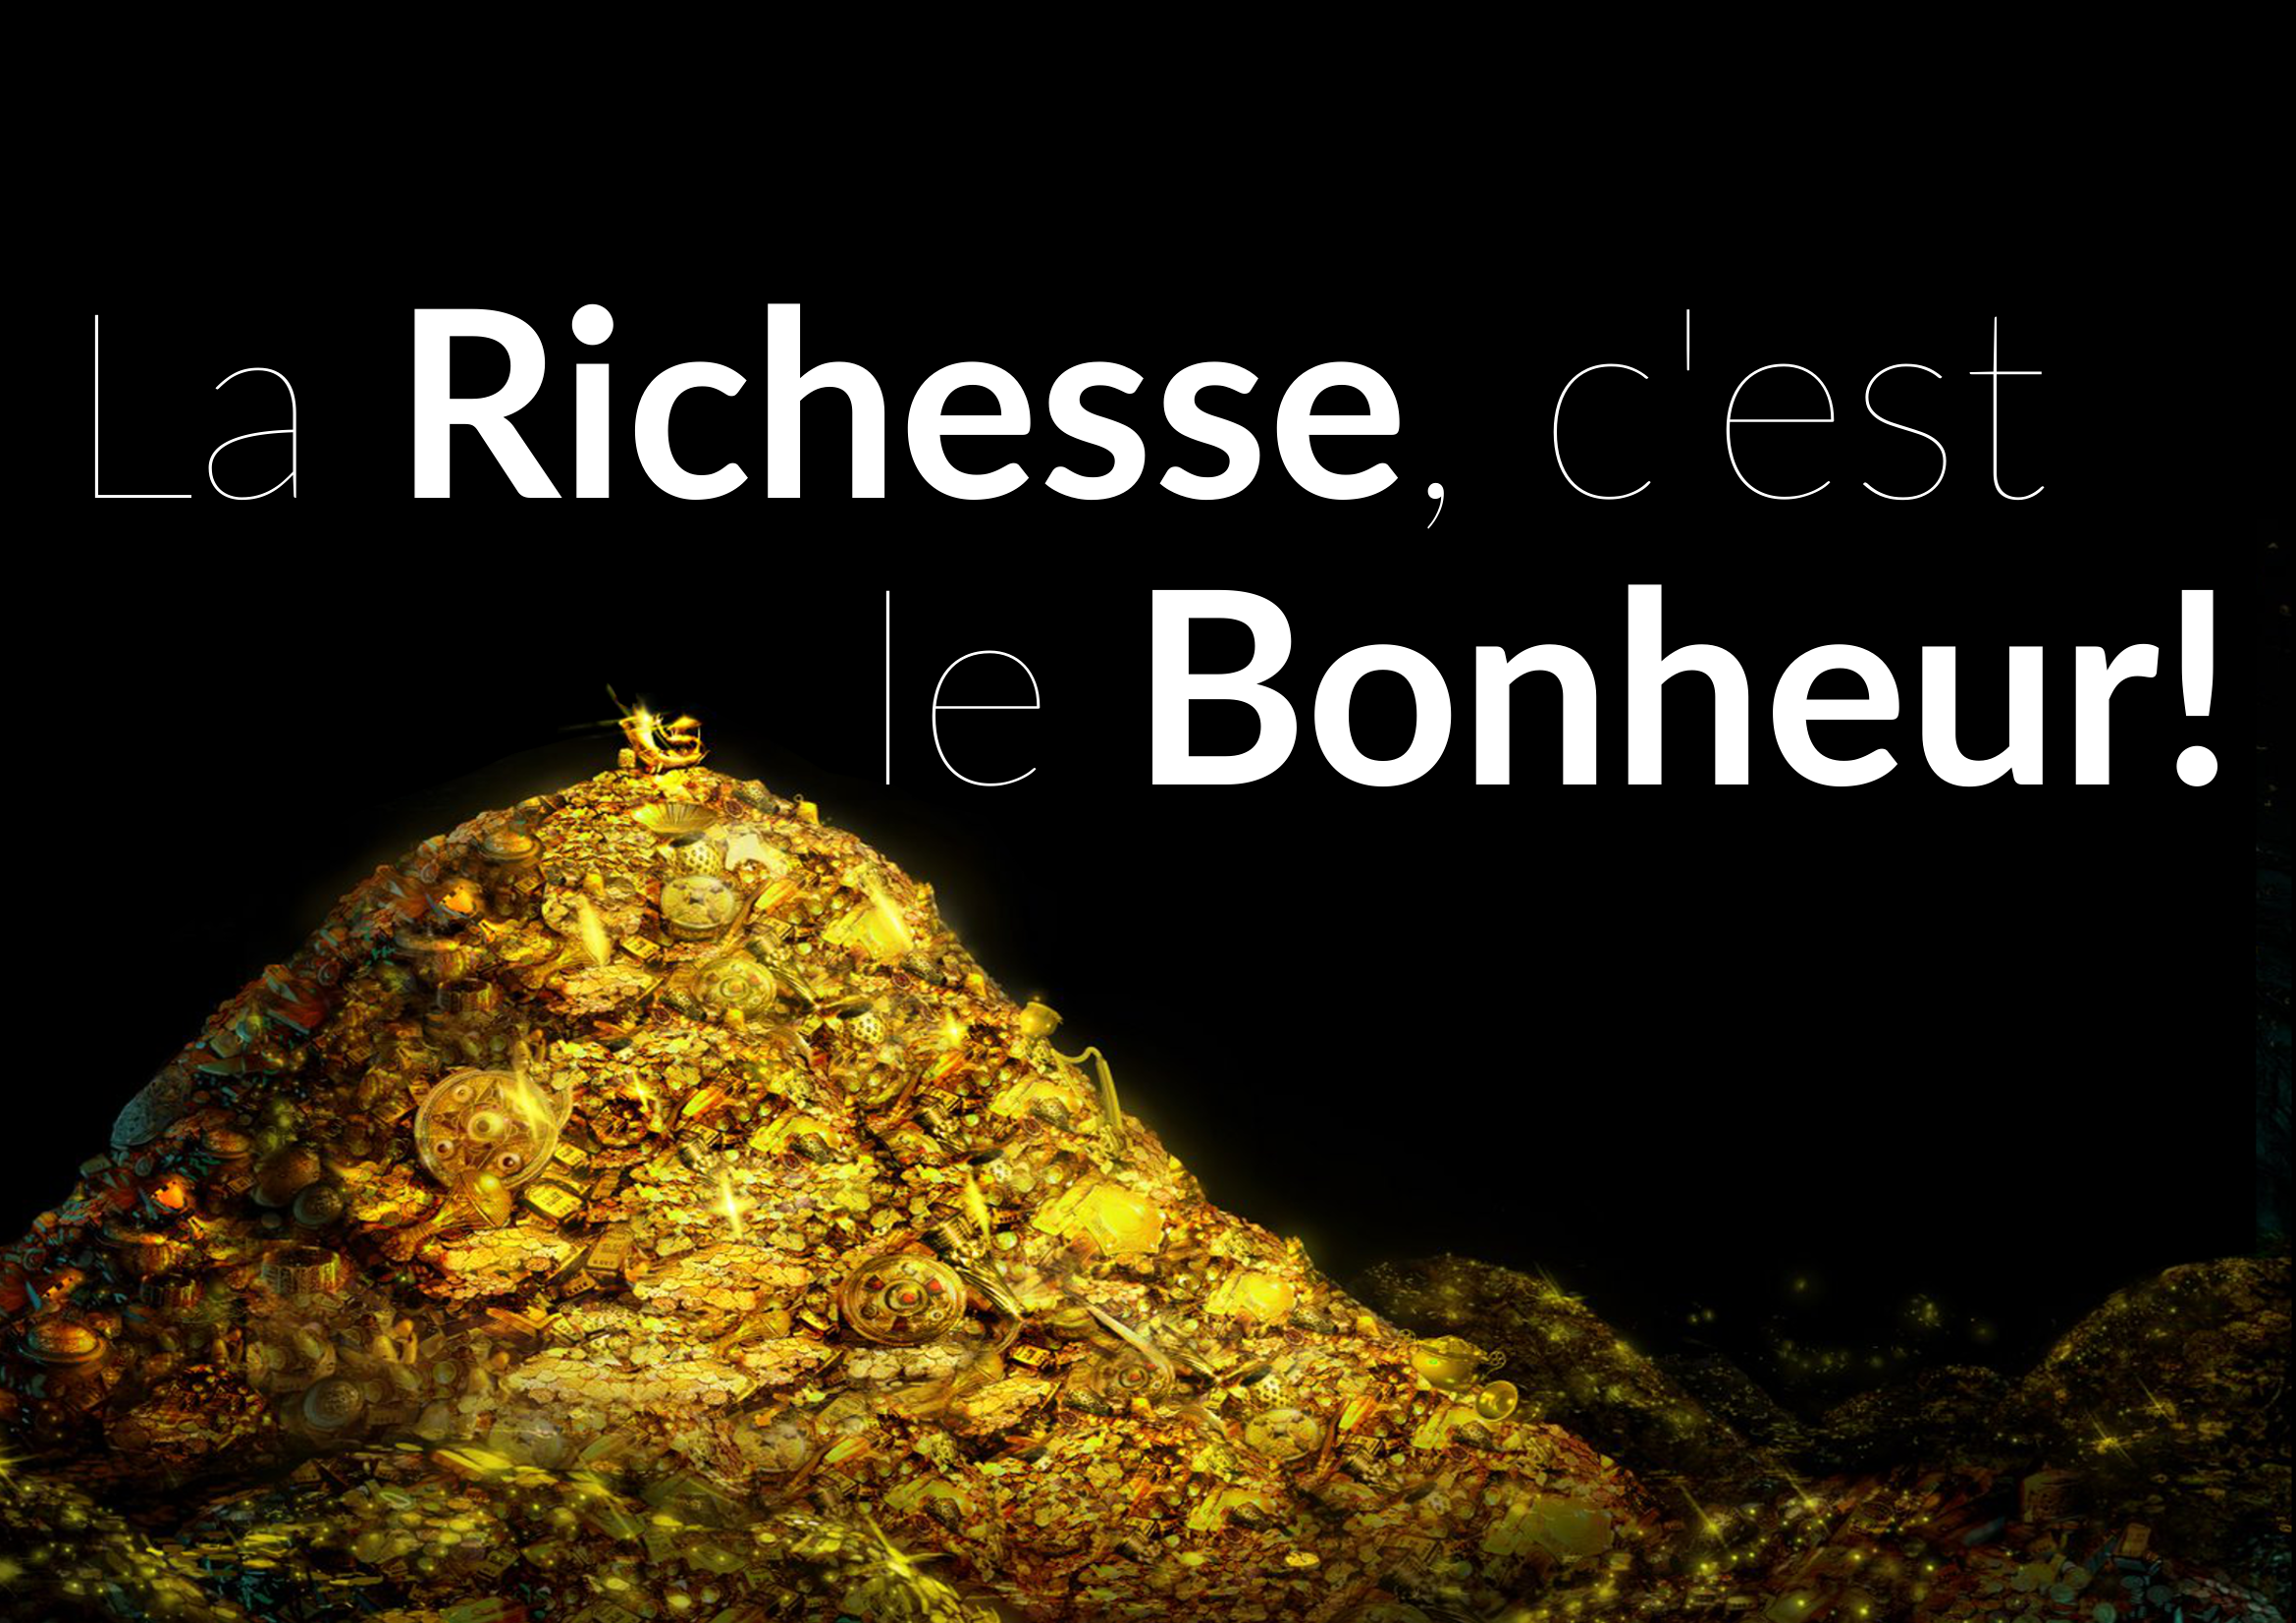
\includegraphics[width=.48\linewidth]{images/Monde/RichesseBonheur.png}}
	\hspace*{.04\linewidth}\subfloat[L'aisance matérielle par le travail]{
\includegraphics[width=.48\textwidth]{images/Monde/travailRichesse.png}}
	\caption{\label{fig:propagandeReligion}Propagande religieuse}
\end{figure}


\subsection{Propagande gaamoniste}
Gaamon utilise également les affiches, parmi d'autres vecteurs, pour répandre ses idées. Un aperçu de ces affiches est donné à la figure \ref{fig:propagandeEtatique}. Les images \ref{subfig:gaamonSauverNature} et \ref{subfig:eliminezTouteNature} répandent les volontés \enquote{anti-naturelles} étatiques, quand à elles, les figures \ref{subfig:industrialisationPourPuissance} et \ref{subfig:electricite} défendent l'industrialisation massive du peuple humain pour la puissance qu'un tel apport fourni.

\begin{figure}[ht!]
	\subfloat[\label{subfig:gaamonSauverNature}Gaamon pour vous sauver de la Nature]{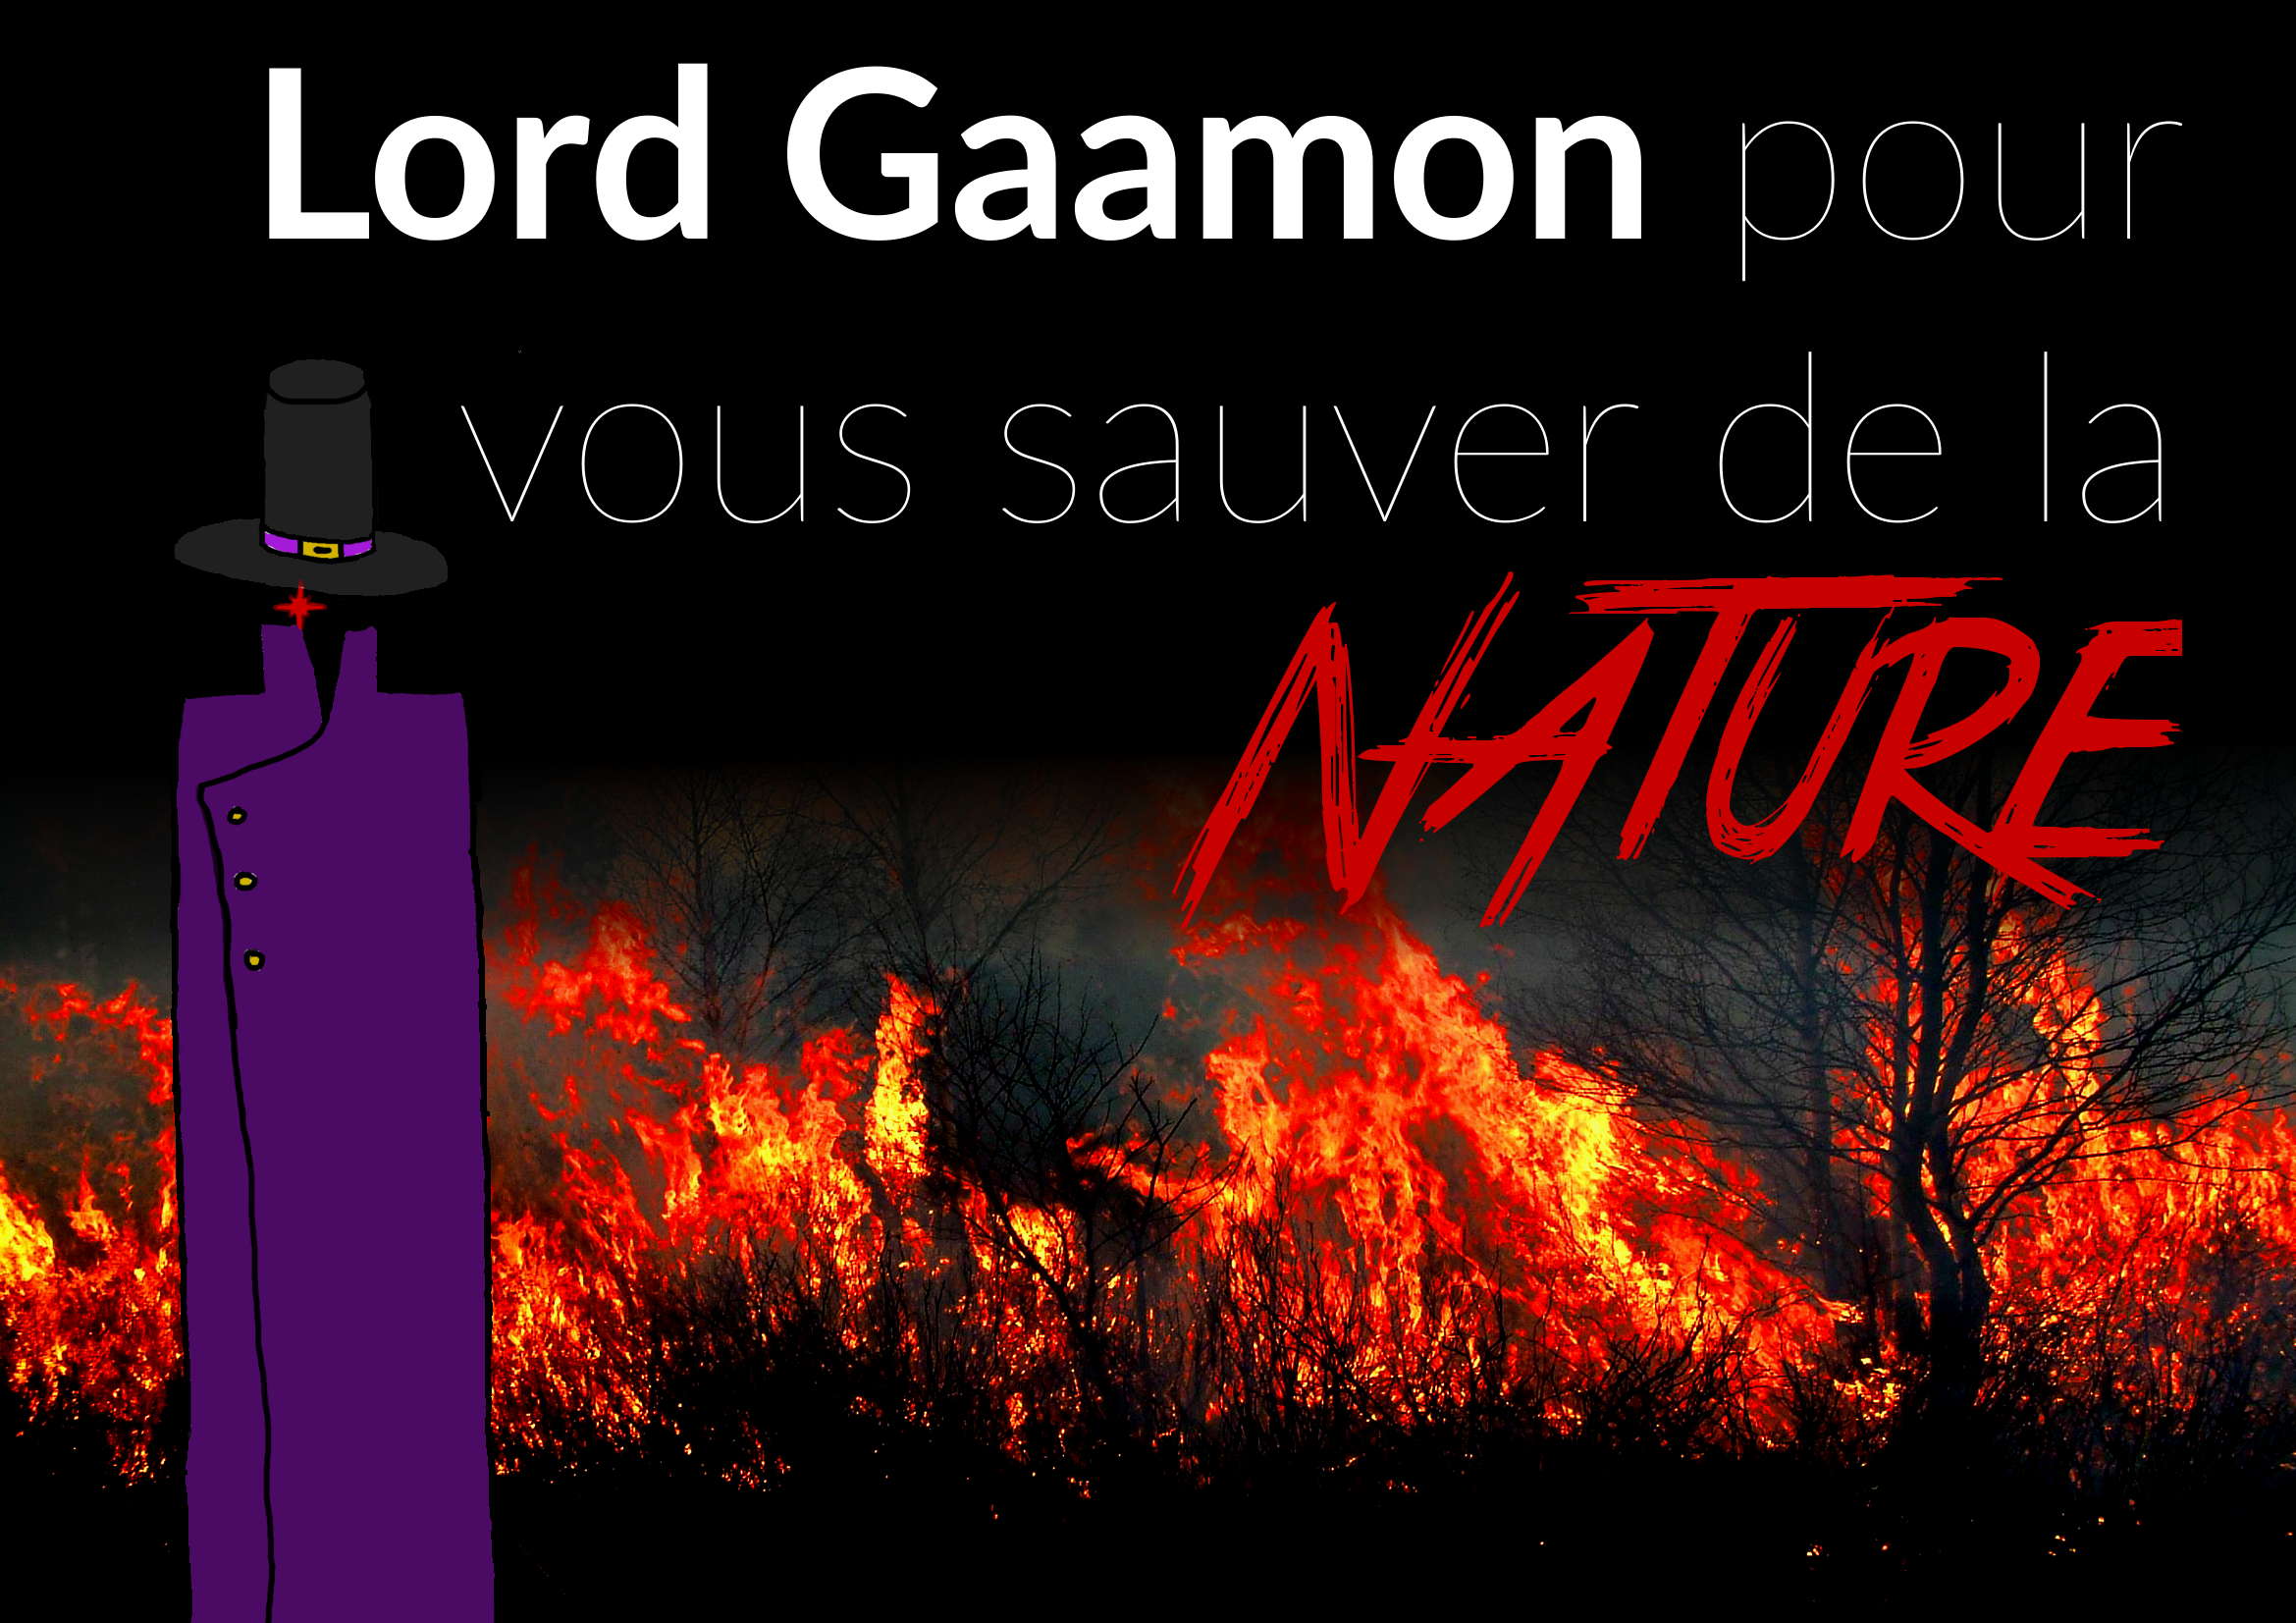
\includegraphics[width=.48\linewidth]{images/Monde/gaamonPourVousSauverNature.png}}
	\hspace*{.04\linewidth}\subfloat[\label{subfig:eliminezTouteNature}Éliminez toute Nature]{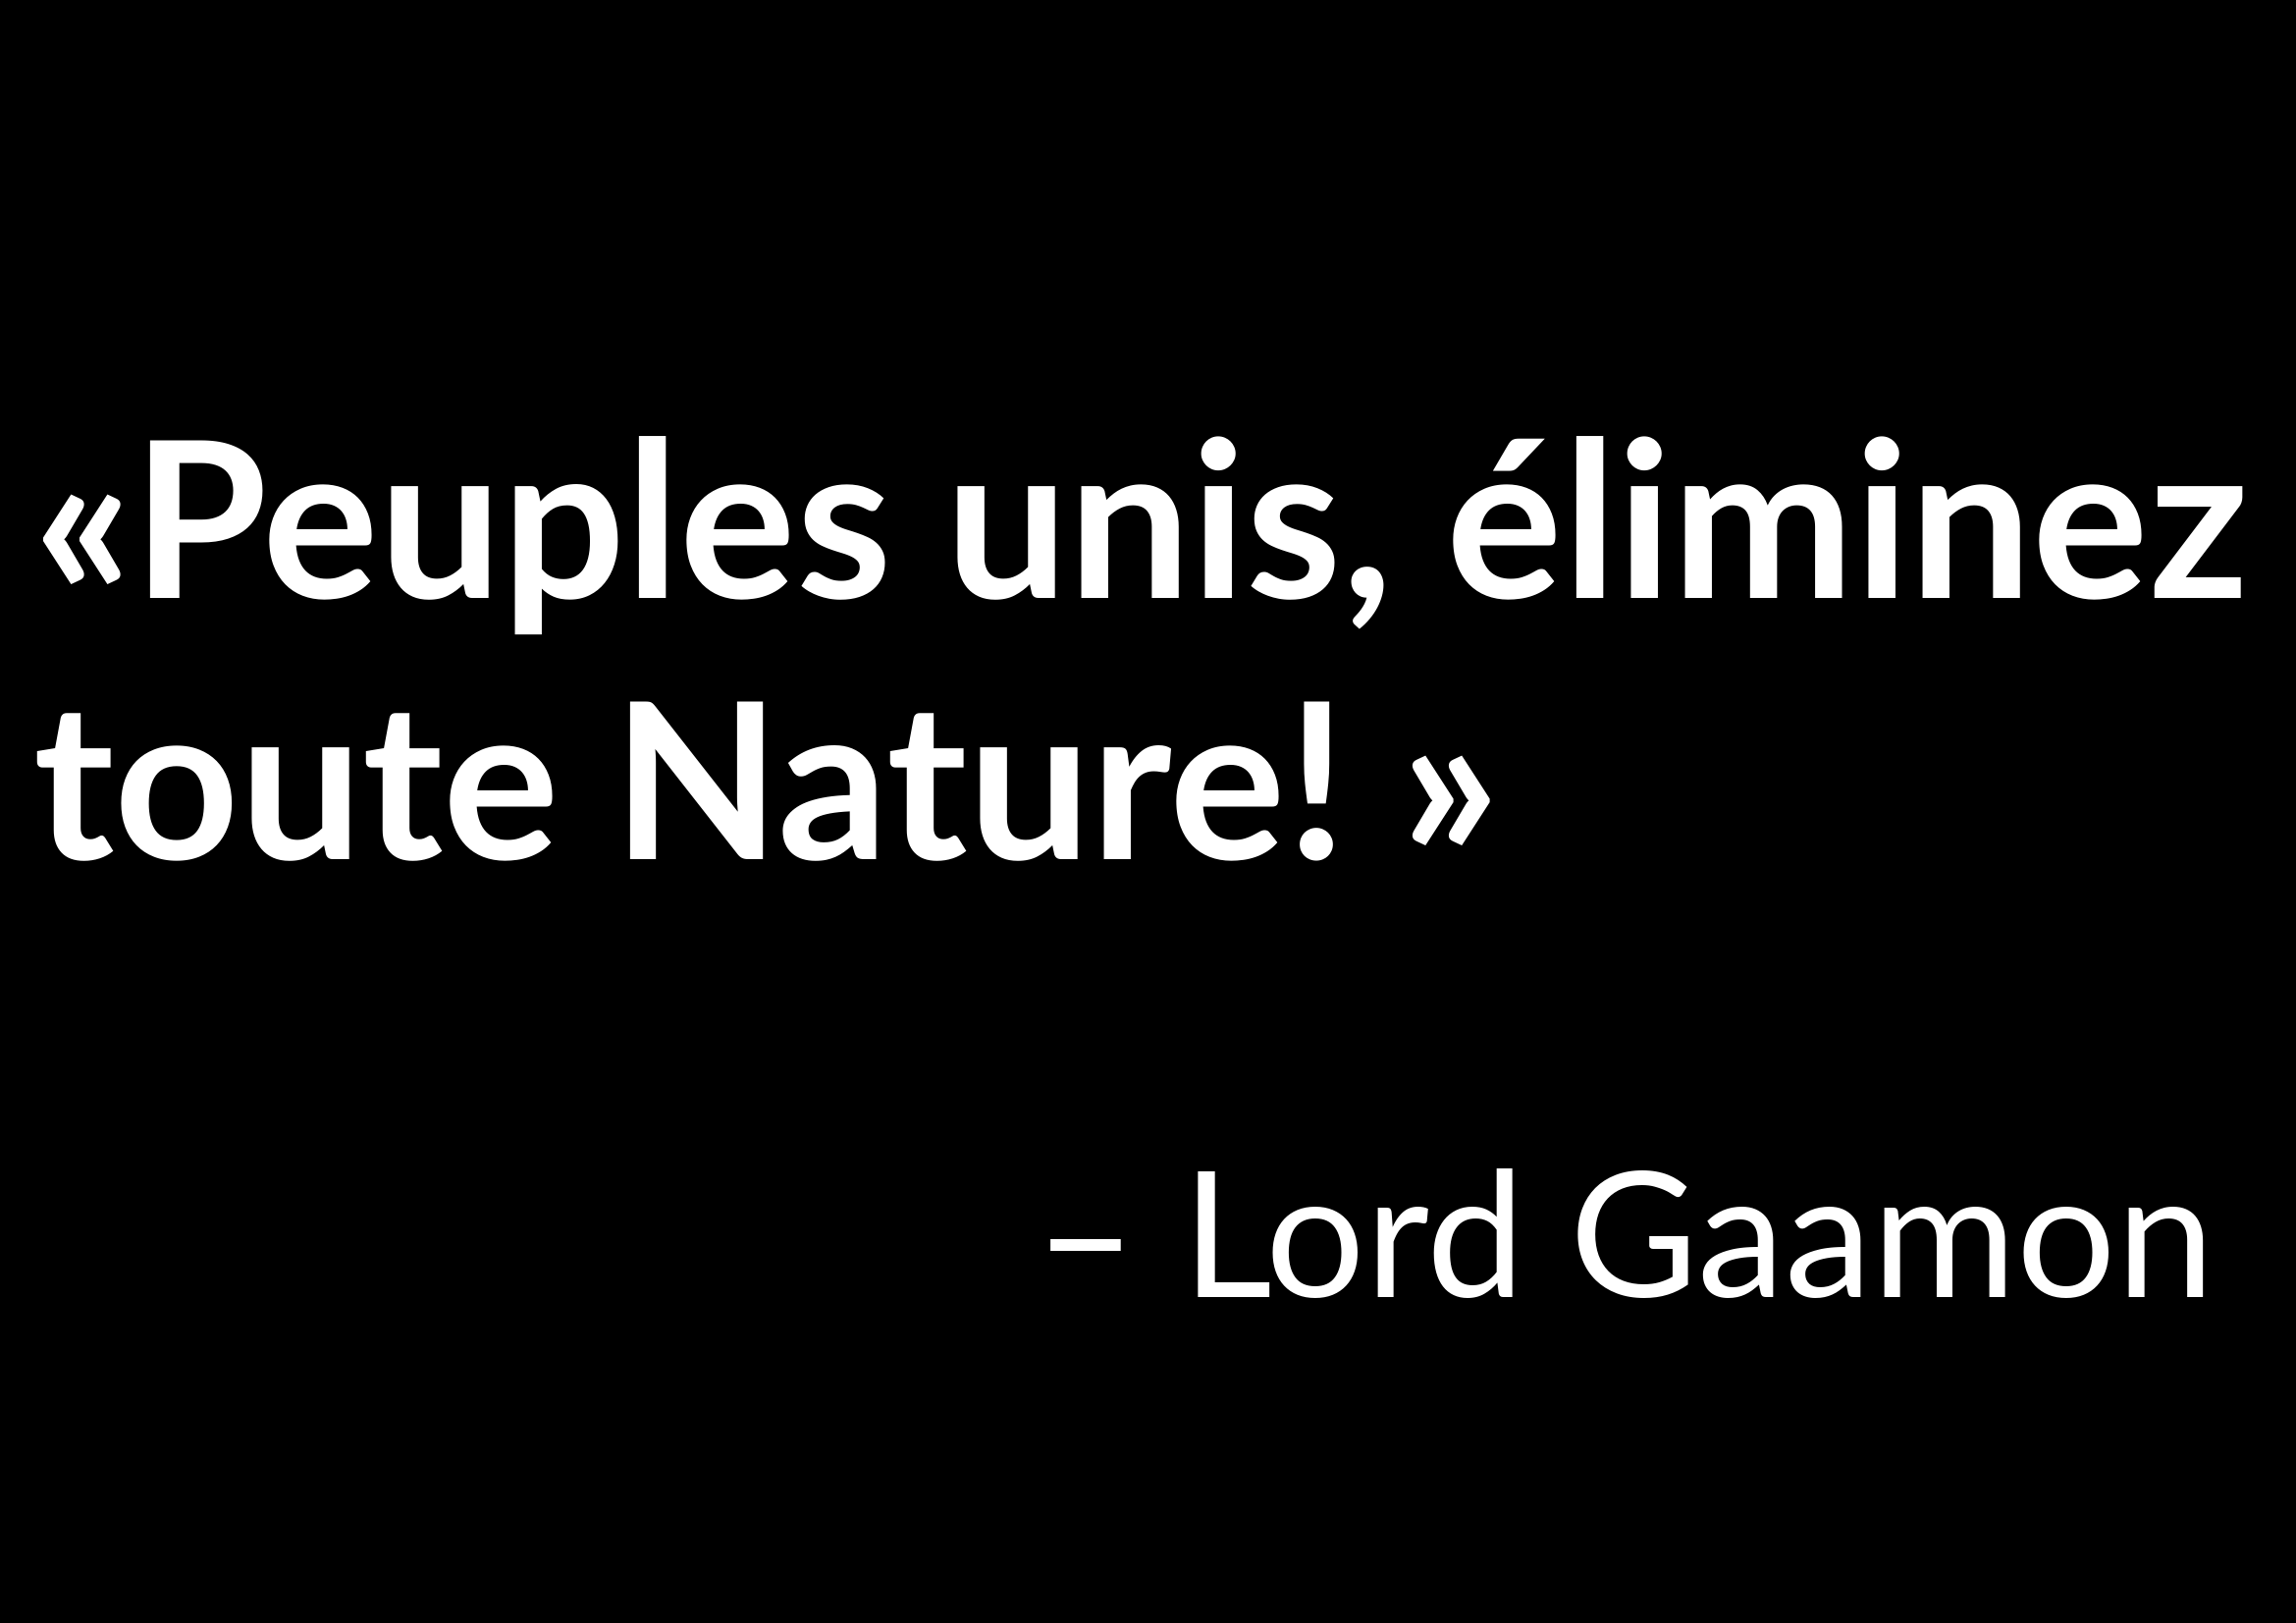
\includegraphics[width=.48\linewidth]{images/Monde/eliminezTouteNature.png}}
	
	\subfloat[\label{subfig:industrialisationPourPuissance}L'industrialisation pour la Puissance]{
\includegraphics[width=.48\textwidth]{images/Monde/industrialisationPourPuissance.png}}
	\hspace*{.04\textwidth}\subfloat[\label{subfig:electricite}Électricité]{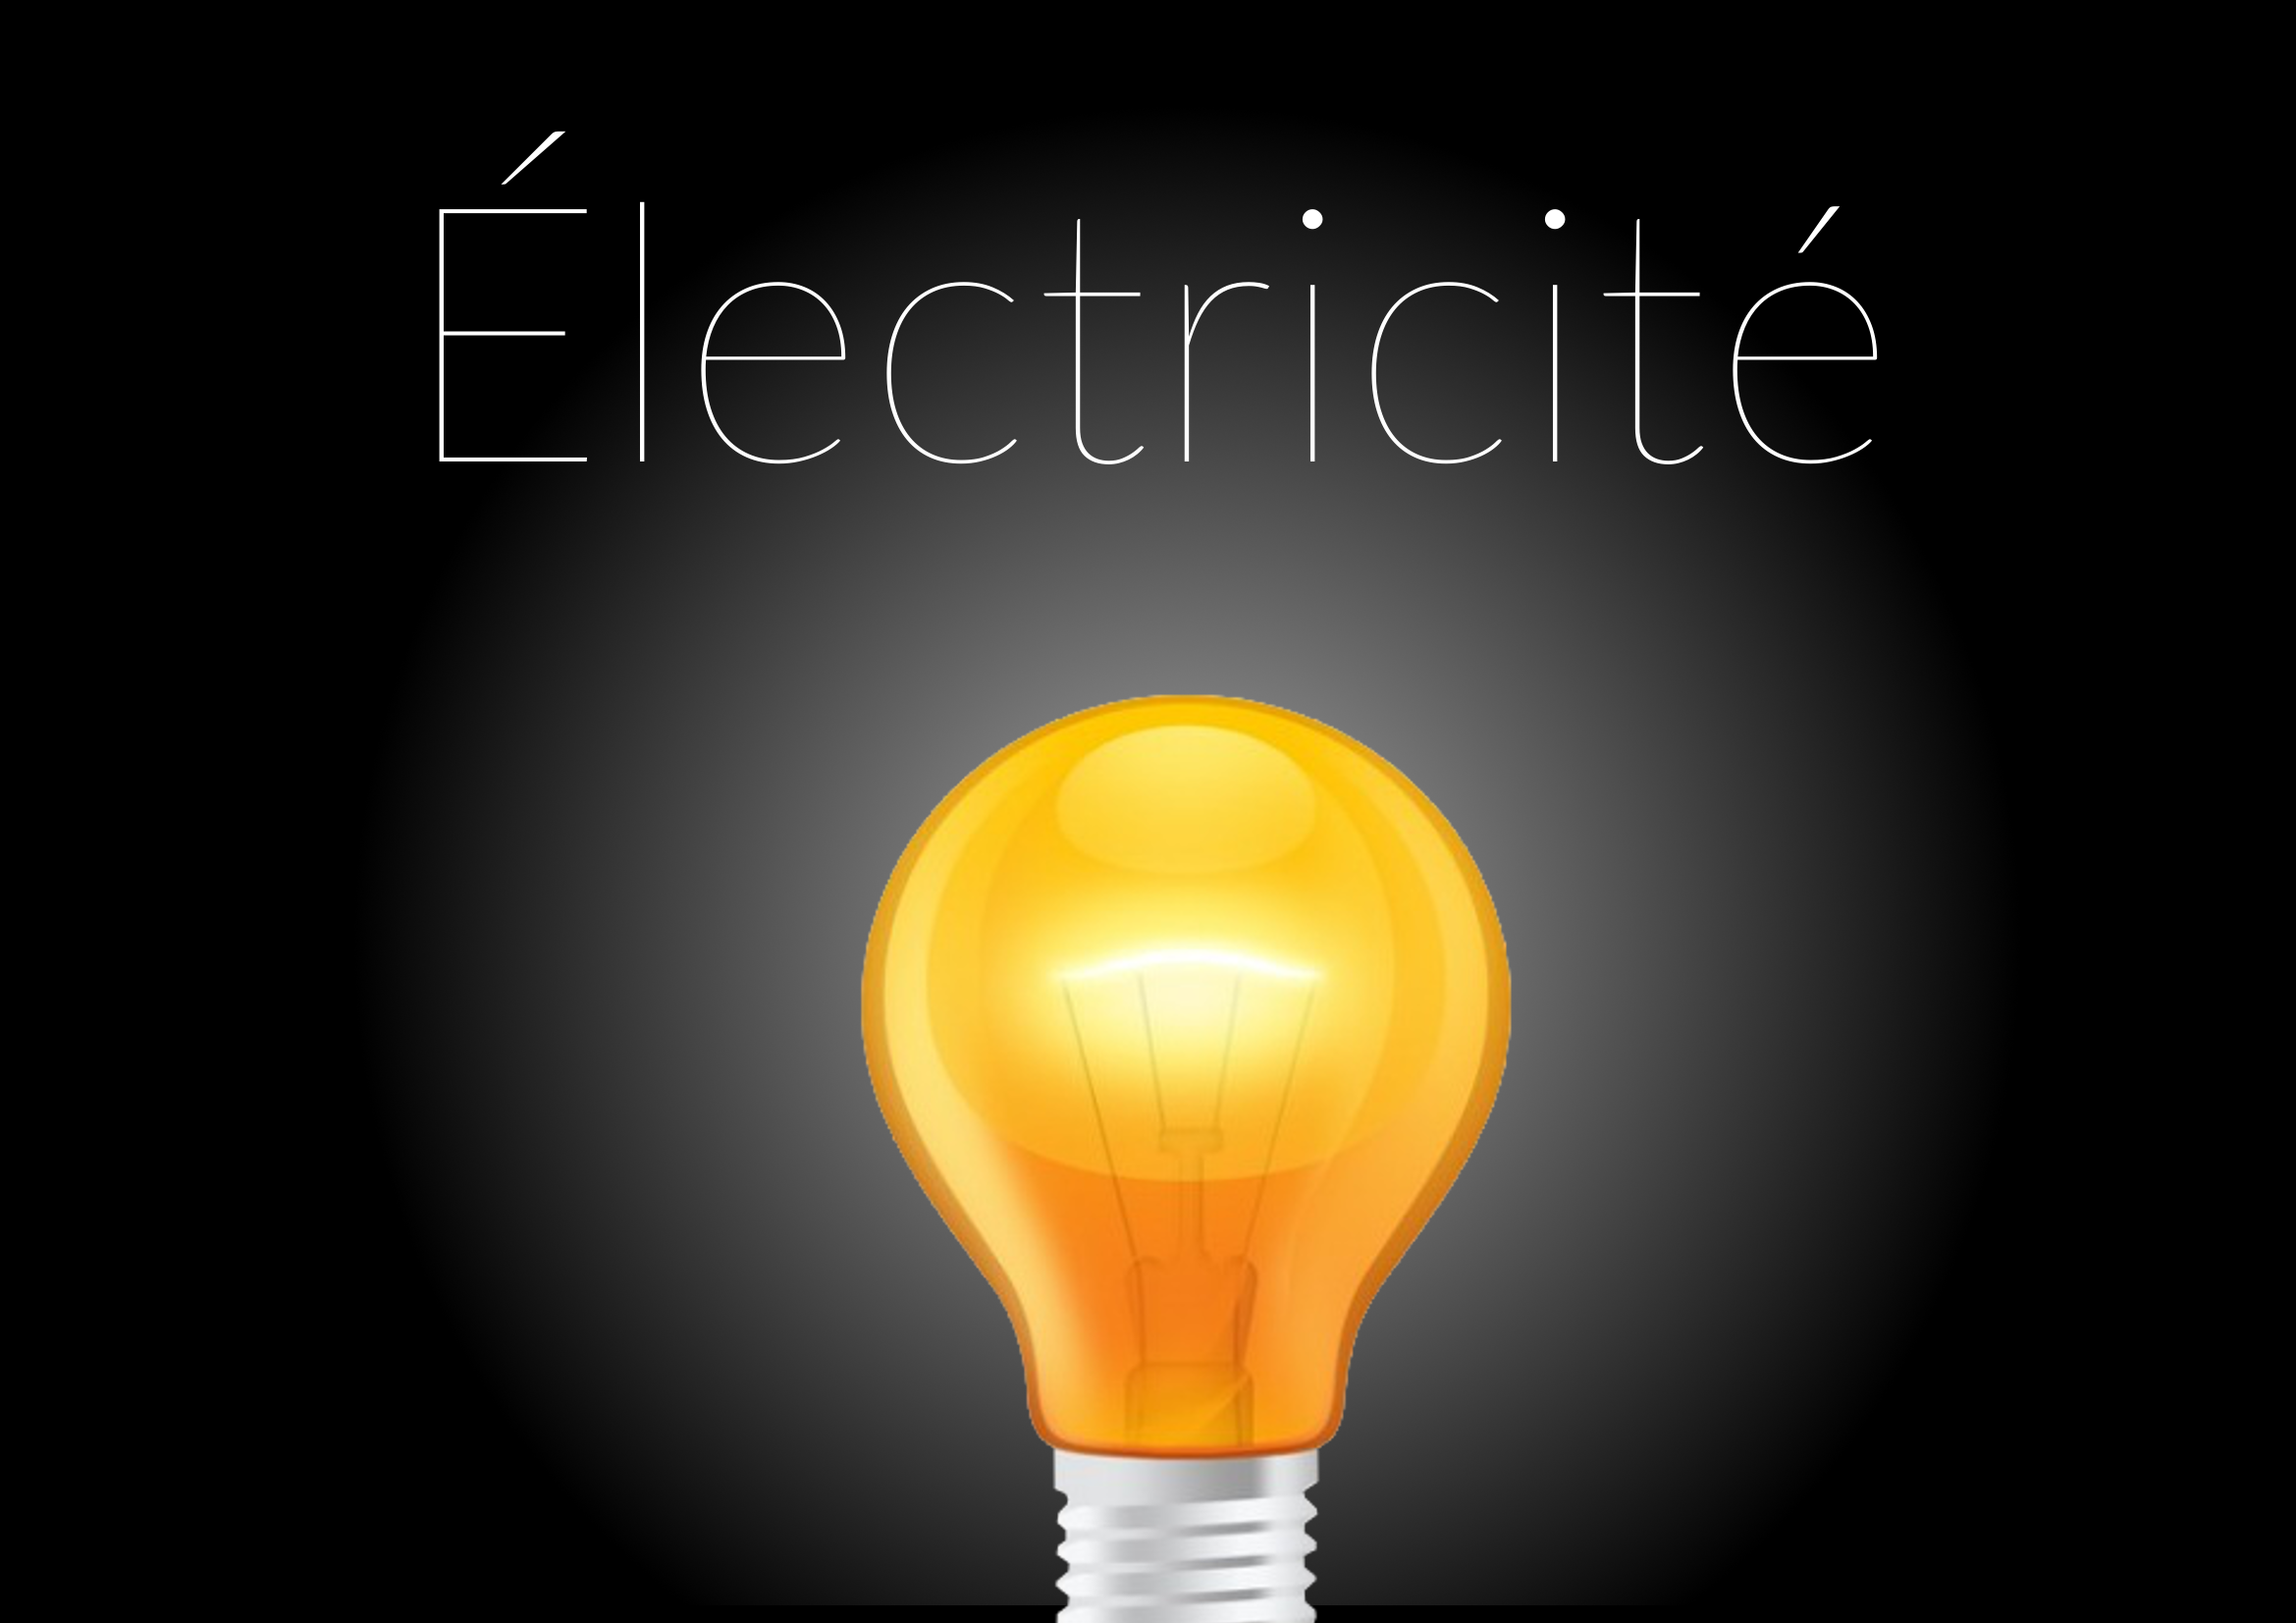
\includegraphics[width=.48\linewidth]{images/Monde/light.png}}
	\caption{\label{fig:propagandeEtatique}Propagande étatique}
\end{figure}



\section{Les \nomNaturels s}
Le nom \enquote{\nomNaturels s} est une anagramme de \enquote{naturels} et pourrait se rapporter à l'adjectif \enquote{tellurique} qui signifie \enquote{de la terre}. Les \nomNaturels s, à l'inverse des Hommes, représentent un peuple pacifique. Ils accordent beaucoup d'importance à la Nature et tentent de vivre en accord avec elle.

Ils sont une espèce différentes des humains. Les humains croyant en la Nature sont, quant à eux, appelés \enquote{Naturels}. Se faire traiter de naturel dans \nomVille\ est une des pires insultes qui soit.


\subsection{Leur histoire}
\label{sec:histoireNaturels}
Les \nomNaturels s étaient, par le passé, le peuple le plus brillant et le plus avancé d'\nomUnivers. Ils avaient trouvé une source d'énergie formidable, l'énergie verte, qui leur permettait de vivre heureux et prospères. L'extraction de cette ressource naturelle était cependant un processus compliqué que seuls les shamans de l'énergie maîtrisaient (voir section \ref{sec:energies}). Grâce à cette source, leurs cités étaient magnifiques, leurs manières connues pour leur raffinement et leur art reconnu pour sa délicatesse.

Ce peuple jouissait d'une prospérité jusque-là sans égale dans l'histoire et répandait sa sagesse, ses connaissances et son amour de la nature de par le monde. L'ascension au pouvoir de Gaamon marqua la fin de cette période; afin d'empêcher la propagation d'un idéal qui mettait la Nature au centre des préoccupations, il fit assassiner les prêtres de l'énergie. Les \nomNaturels s se retrouvèrent subitement privés de leur source vitale -- l'énergie verte -- sans protection et virent leur civilisation s'effondrer brutalement.

Les \nomNaturels s vivent maintenant reclus sur de hauts plateaux, cachés de la haine ainsi que des persécutions de Gaamon et rêvent de leur gloire passée. Si leur idéologie d'amour envers la Nature perdure, cette civilisation décline de jour en jour.



\section{Énergies}
\label{sec:energies}
Les énergies sont un élément clé de ce monde, elles déterminent quels peuples survivront et quels seront ceux qui disparaîtront. C'est un parallèle de notre dépendance à l'énergie. En effet, on ne peut plus imaginer aujourd'hui vivre sans électricité. À \nomUnivers, les sources d'énergies sont diverses et représentatives des peuples.

\subsection{Humains}
Chez les Humains, l'énergie est tirée du charbon pour créer de la vapeur et de l'électricité. C'est une source très polluante. La couleur qui lui est attribuée est le rouge du feu des hauts fourneaux et le noir de la fumée nauséabonde qui remplit le ciel de \nomVille. Elle fait partie intégrante du Steampunk, caractéristique de ce peuple.

\subsection{\nomNaturels s}
À l'inverse, les \nomNaturels s ont exploité l'énergie des arbres, appelée énergie verte. Les plantes fournissaient un apport énergétique et, en contrepartie, les \nomNaturels s portaient une attention toute particulière à leur santé, reproduction, protection et longévité. Une symbiose existait entre les \nomNaturels s et la Nature, un équilibre grandement profitable autant pour l'un que l'autre des partis. L'énergie verte était extraite dans la grande salle, dont l'accès était réservé aux grands shamans de l'énergie. Ils étaient les seuls à pouvoir en maîtriser le fonctionnement complexe. Si ce secret était aussi bien gardé, c'est que cette énergie très puissante, extraite en trop grandes quantités, aurait pu causer la mort de milliers d'arbres et animaux. Un tel cas de figure était à craindre car la Nature se serait retournée contre les personnes ayant abusé de ses ressources et, dans sa fureur, aurait annihilé les profiteurs. Les \nomNaturels s, craignant une pareille situation, s'en étaient prémunis en cachant les mécanismes de la grande salle pour ne les révéler qu'aux seuls élus, les shamans.

Cette énergie pouvait également être maîtrisée, dans une moindre mesure, à titre personnel. Les personnes dotées de telles capacités pouvaient alors lancer des \enquote{sorts}. Ceci est un des éléments clé du gameplay (voir section \ref{sec:sorts}). On pourrait comparer l'énergie verte à de la magie mais cela ne serait pas très judicieux: l'énergie verte n'est ni illimitée, ni gratuite. L'utiliser de façon disproportionnée signifie tuer toute vie alentour. Et si la Nature est généreuse elle peut aussi refuser de donner son bien, voire punir ceux qui en abusent. Il est également possible de l'extraire de soi-même, mais une fois de plus, la réalisation d'une telle opération est dangereuse car elle peut causer la mort de l'exécutant.

Depuis la disparition mystérieuse des shamans (voir section \ref{sec:histoireNaturels}), les \nomNaturels s ont perdu le secret de l'énergie verte. Ils utilisent donc les énergies hydraulique et éolienne, facilement disponibles dans les montagnes où ils vivent. Elles sont cependant bien moins puissantes que l'énergie verte et ne leur permettent de loin pas les miracles qu'ils pouvaient accomplir avec la première.

\section{Bestiaire}
\label{sec:Bestiaire}
L'univers d'\nomUnivers\ est peuplé de créatures. Du point de vue des genres, ce monde est un croisement entre la science-fiction et la \anglicisme{Fantasy}.

\subsection{Créatures humaines}
Les sbires de Gaamon sont des créatures nommées \textit{Gnobols}. Il existe beaucoup de variantes de la créature \enquote{de base}, mais ils sont tous équipés d'un chapeau duquel une fumée noire s'échappe .Certains, cependant, auront une armure quand d'autres seront munis d'un arc ou d'un fusil.

\begin{figure}[h!]
	\center
	
\includegraphics[width=.3\textwidth]{images/Monde/Gnobol.png}
	\caption{Gnobol}
\end{figure}

\subsection{Personnalisation de la Nature}
\label{sec:personnalisationNature}
Dans \nomJeu, la Nature est personnalisée par trois esprits, chacun représentatif d'un aspect de la Nature qui définit leur apparence:

\begin{table}[ht!]
	\newlength{\tableLength}
	\setlength{\tableLength}{\textwidth+2.3cm}
	
	\hspace{-2.3cm}
	\begin{tabu} to \tableLength {l l X X X l}
		\rowfont{\bfseries\sffamily\leavevmode\color{white}}
		\rowcolor{mainColor}
		& Esprit & Description & Mots-clé & Apparence & \\
		& Leo & Il est la destruction renouvelatrice, à la fois créateur et destructeur & Massif, sans distinction, abrupte, rapide, mort génératrice de vie & Golem, de pierre et de lave en bas, de pierre et d'eau en haut, avec un duvet de plante sur les épaules & \\
		& Tamund & Il est l'intelligence aveugle, l'évolution lente & Évolution, lent, ciblé, mort des plus faibles & Grand séquoia aveugle & \\
		& Tia & Elle est la vivacité sauvage et profite parfois sans pitié & Sauvage, vif, rapide, profiteur, sans-pitié, survie du plus adapté et mort des plus faibles & Écureuil avec des runes sur le dos & \\
	\end{tabu}
	
	\caption{Les trois esprits et leurs caractéristiques}
\end{table}

\begin{figureWithNotes}[ht!]
	%\savenotes
	\center
	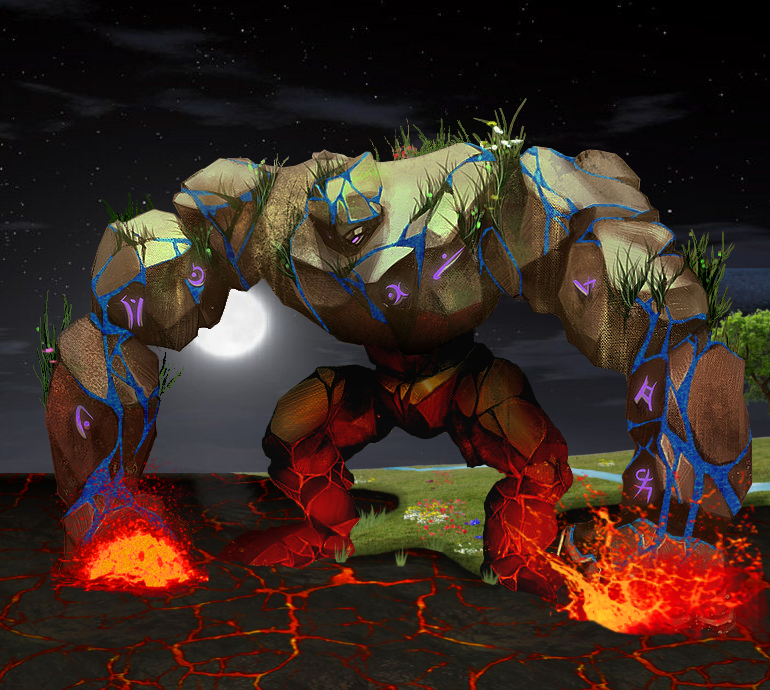
\includegraphics[width=\textwidth]{images/Monde/Leo/Leo.png}
	\caption{Une esquisse de Leo, basée sur le travail original de Sinto-risky {\cite{StoneGolem_Sinto-risky}}}
	%\spewnotes
\end{figureWithNotes}
